\documentclass[12pt, letterpaper]{article}
\usepackage{graphicx} % Required for inserting images
\usepackage{hyperref}
\usepackage{listings}
\usepackage{amssymb}
\usepackage{amsmath}
\usepackage[english]{babel}
\usepackage{amsfonts}
\usepackage{nicefrac, xfrac}
\usepackage[utf8]{inputenc}
\usepackage{mathtools}
\newcommand{\acc}{\\\hphantom{}\\}
\usepackage[dvipsnames]{xcolor}
\usepackage[titles]{tocloft} % Optional: Better control of the table of contents

\definecolor{light-gray}{gray}{0.95}
\newcommand{\code}[1]{\colorbox{light-gray}{\texttt{#1}}}
\newcommand{\codee}[1]{\colorbox{white}{\texttt{#1}}}
\usepackage[paper=a4paper,left=20mm,right=20mm,bottom=25mm,top=25mm]{geometry}
\renewcommand{\labelenumii}{\arabic{enumi}.\arabic{enumii}}
\renewcommand{\labelenumiii}{\arabic{enumi}.\arabic{enumii}.\arabic{enumiii}}
\renewcommand{\labelenumiv}{\arabic{enumi}.\arabic{enumii}.\arabic{enumiii}.\arabic{enumiv}}
\newcommand{\id}{{\hphantom{ident}}}
\newcommand{\vincolo}[1]{\colorbox{Orange}{$[$\text{#1}$]$}}
\title{\textbf{Out!}}

\date{}

\begin{document}

\maketitle

\tableofcontents 
\newpage
\section{Requisiti}
\begin{verbatim}
    1. Utente
        1.1 Cf
        1.2 Nome
        1.3 Cognome
    
    2. Prenotazione 
        2. DataOra
    
    3. Posto 
        3.1 Fila
        3.2 Colonna
        3.3 Settore
    
    4. Sala 
        4.1 Nome
        4.2 PostiTotali
    
    5. Sede
        5.1 Indirizzo
    
    6. Citta
        6.1 Nome

    7. Nazione
        7.1 Nome
    
    8. Rappresentazione
        8.1 DataOra
        8.2 DurataOre
    
    9. Spettacolo
        9.1 Titolo
        9.2 Tipologia
        
    10. Genere
        10.1 Nome
    
    11. Artista
        11.1 Nome
        11.2 Cognome


\end{verbatim}
\newpage\section{UML}
\begin{center}
    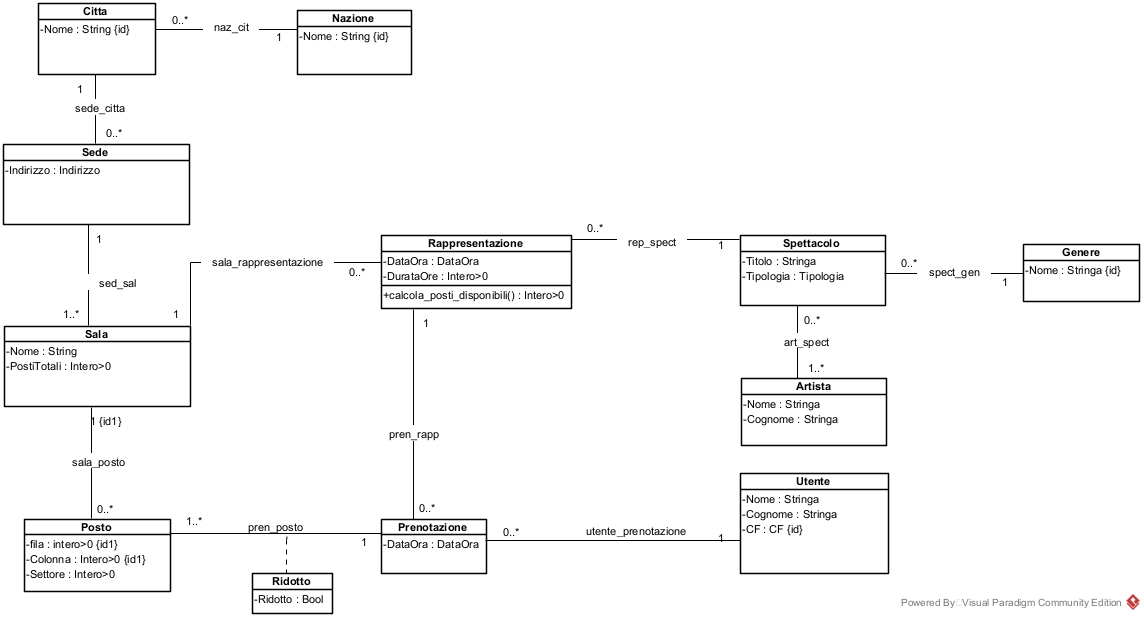
\includegraphics[width=1\textwidth ]{Images/UML.jpg}
\end{center} \newpage
\section{Tipi di Dato}
\begin{itemize}
    \item Tipologia= \{ "Film", "Rappresentazione Teatrale", "Concerto" \}
    \item CF = Stringa secondo Regex $[A-Z]\{6\}[0-9]\{2\}[A-Z][0-9]\{2\}[A-Z][0-9]\{3\}[A-Z]$
\end{itemize}

\section{Vincoli Esterni}
\begin{itemize}
   \item $[V.Prenotazione.Data]$ \acc
   Non è possibile prenotare per uno spettacolo passato \\
   $\forall p,d,a,g Prenotazione(p) \land DataPrenotazione(p,d) \land Adesso(a) \land GiornoOdierno(a,g)\rightarrow g>d $
   \item $[V.Rappresentazione.Simultanea]$ \acc 
   Non più di 1 rappresentazione per sala nello stesso momento \\
   $\forall r,s,g,h,d,r',s',g',h',d'$\\ $Rappresentazione(r) \land Sala(s) \land SalaRappresentazione(r,s) \land giornoRappresentazione(r,g) \land oraGiornoRapp(r,g,h) \land DurataRappresentazione(r,d) \land$ \\
   $Rappresentazione(r') \land Sala(s') \land SalaRappresentazione(r',s') \land giornoRappresentazione(r',g') \land oraGiornoRapp(r',g',h') \land DurataRappresentazione(r',d') \land$\\
   $ r!=r' s=s' g=g' \rightarrow (h+d<h' \lor h> h'+d')$
   \item $[V.Sala.Posti]$ \acc
   N PostiPrenotazione $<=$ Sala.PostiTotali\\
   $\forall s,p Sala(s)\and calcola\_posti\_liberi(s,p)\\$ $p>0 $
   \item $[V.Posto.PostiDiversi]$\acc 
   Non possono esserci due posti uguali nella stessa sala legati a due prenotazioni diverse\\
   $\forall ps Posto(ps)\rightarrow \not \exists p1,p2,r Prenotazione(p1) \land Prenotazione(p2) \land pren\_posto(p1,ps) \land pren\_posto(p2,ps) \land pren\_rap(p1,r) \land pren\_rap(p2,r) \land p1!=p2$\\
   \item $[V.Prenotazione.PostoInSala]$\acc 
   Se un utente prenota per una rappresentazione e un determinato posto esso si trova nella sala della rappresentazione\\
   $\forall p,r,ps,s Prenotazione(p) \land Rappresentazione(r) \land pren\_rap(p,r) \land pren\_posto(p,ps) \land \\ SalaRappresentazione(s,r)\rightarrow sala\_posto(ps,s)$
\end{itemize}\newpage
\section{Specifica Classi}
\subsection{Classe Rappresentazione}
\subsubsection{calcola\_posti\_disponibili(): Intero}
\begin{itemize}
    \item PreCondizioni: nessuna
    \item Modifiche al livello estenzionale: nessuna
    \item PostCondizioni:\\
        $\forall s,p Sala(s)\and PostiSala(s,p)\\$ $P=\{ (p,s) Posto(p) \land Sala(s,p) \} $\\
        Result è uguale a $ PostiSala - |P|$

\end{itemize}
\section{Use-Case}
\subsection{Diagramma}
\begin{center}
    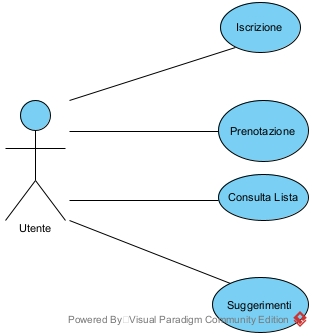
\includegraphics[width=1\textwidth ]{Images/UseCase.jpg}
\end{center} \newpage
\subsection{Specifica Use-Case}
\subsubsection{Iscrizione}
\begin{verbatim}
    iscrizione(n: Stringa, c: Stringa, cf: CF): Utente
    PreCondizioni: nessuna
    PostCondizioni:
        Modifica il livello estensionale quindi Min!=Mout.
        Elementi in D aggiunti: p
        Elementi in D rimossi: nessuno
        Oggetti aggiunti: 
            -Utente(p)
                -nome(p,n)
                -cognome(p,c)
                -CF(p,cf)
        Oggetti rimossi: nessuno
        result = p
\end{verbatim}
\subsubsection{Prenotazione}
prenotazione(u: Utente, r: Rappresentazione, n: Intero, s: Intero): Prenotazione
    \begin{itemize}
        \item PreCondizioni:\\ $\exists Utente(u) \land  Rappresentazione(r) \land SalaRappresentazione(s,r) \land calcola\_posti\_liberi(s,p) \ge n$.
        \item PostCondizioni:
    \end{itemize}
\begin{verbatim}
    Modifica il livello estensionale quindi Min!=Mout.
    Elementi in D aggiunti: p
    Elementi in D rimossi: nessuno
    Oggetti aggiunti: 
        - Prenotazione(p)
        - pren_rap(p,r)
        - utente_prenotazione(p,u)
        - Sia Sala(s) tale che SalaRappresentazione(r,s)
        - Vengono creati n oggetti pren_post(p)
\end{verbatim}
\newpage
\subsubsection{Consulta Lista}
$consulta\_lista(t:Stringa, g: Stringa, d: Data): Insieme$
\begin{itemize}
    \item PreCondizioni: \\ $\exists Rappresentazione(r) \land TipoRappresentazione(r,t) \land GenereRappresentazione(r,g) \land GiornoRapp(r,d)$\\
    \item PostCondizioni: 
\end{itemize}
\begin{verbatim}
    Non modifica il livello estensionale quindi Min=Mout.
    Elementi in D aggiunti: nessuno
    Elementi in D rimossi: nessuno
\end{verbatim}
    - Sia R=$\{r Rappresentazione(r) \land TipoRappresentazione(r,t) \land GenereRappresentazione(r,g) \land GiornoRapp(r,d)\}$
    Result = R

\subsubsection{Suggerimenti}
$proponi\_suggerimento(): Insieme$
\begin{itemize}
    \item PreCondizioni: nessuna
    \item PostCondizioni:
\end{itemize}
\begin{verbatim}
    Non modifica il livello estensionale quindi Min=Mout.
    Elementi in D aggiunti: nessuno
    Elementi in D rimossi: nessuno
    - Sia Utente(this)\end{verbatim}
    - Sia $R= \{Rappresentazione(r) | utente\_pren(this,p) \land pren\_rap(p,r)\}$\\

    - Sia UltimaRappresentazione(r) la rappresentazione più recente in R\\
    - Sia GenereRappresentazione(r, g)\\
    - Sia S =$ \{Rappresentazione(r) | GenereRappresentazione(r,g) \land GiornoRapp(r,d)$ \\
        $\land adesso(a) \land GiornoAttuale(ga) \land d>ga+7\}$\\
    Result = S
    \newpage




Arrivati a questo punto la fase di \textbf{Analisi} è \textbf{finita}.
\section{Ristrutturazione}
\subsection{Diagramma UML ristrutturato}
\begin{center}
    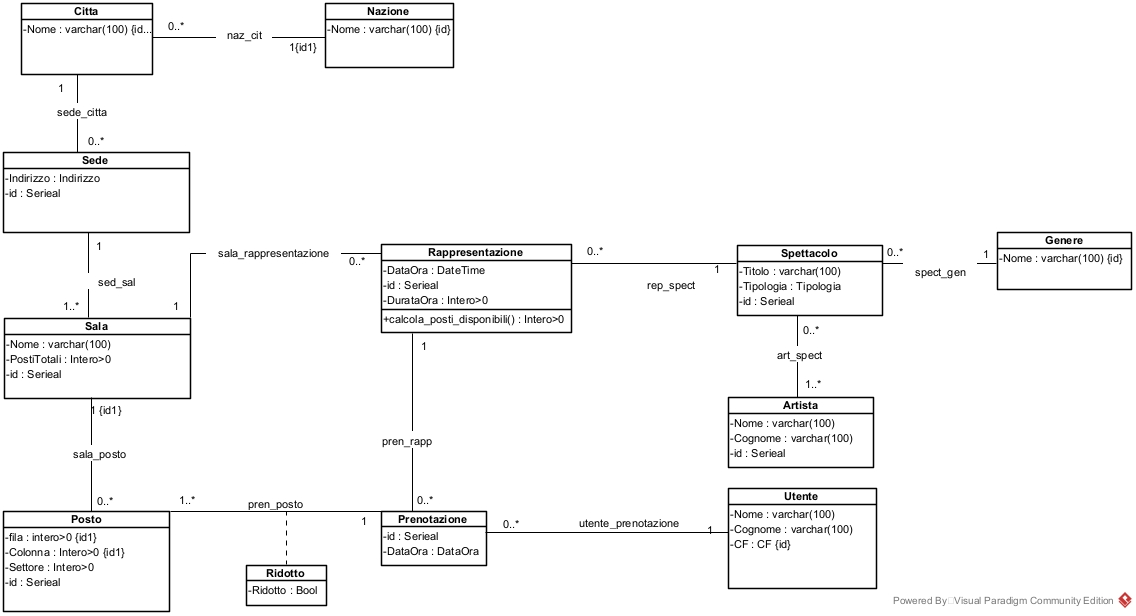
\includegraphics[width=1\textwidth ]{Images/UMLRistrutturato.jpg}
\end{center} \newpage
\textbf{Modifiche sulle generalizzazioni effettuate:}
Non è stato necessario eseguire nessuna modifica sulle generalizzazioni.


\subsection{Tipi e Domini}
\subsubsection{Tipi}
\begin{itemize}
    \item create type Tipologia as enum= $\{"Film", "Rappresentazione Teatrale", "Concerto"\}$
    \item create type Indirizzo= $\{via: varchar, civico: Intero \ge 0\}$
\end{itemize}
\subsubsection{Domini}
\begin{itemize}
    \item create domanin $intero>0$ as Integer check($value \ge 0$)
    \item create domain CF as varchar check($value \text{rispetta la regex} [A-Z]\{6\}[0-9]\{2\}[A-Z][0-9]\{2\}[A-Z][0-9]\{3\}[A-Z]$)
\end{itemize}
\subsection{Vincoli Esterni}
Non sono stati inseriti nuovi vincoli esterni.
\subsection{Use Case}
Gli use case non violano la nuova ristrutturazione.
\newpage
\subsection{Traduzione diretta del diagramma UML delle classi ristrutturato}
Saranno scritte tutte le tabelle da creare:
\begin{verbatim}
- Nazione(_nome_: varchar)

- Citta(_nome_: varchar, _nazione_: varchar)
    fk: nazione references Nazione(nome)

-Sede(_id_: Serieal, Inidirizzo: Indirizzo, _citta_: varchar)
    fk: citta references Citta(nome)

-Sala(_id_: Serial, Nome: varchar, PostiTotali: intero, Sede: Intero)
    fk; sede references Sede(id)

-Posto(_id_: Serial, Fila: Intero>0, Colonna: Intero>0, 
        Settore: Intero>0, Sala: Intero)
    unique(Fila, Colonna, Settore, Sala)
    fk: sala references Sala(id)

-Rappresentazione(_id_: Serial, TDataOra: DateTime, 
                  DurataOre: Intero>0, Sala: Intero, Spettacolo: intero>0)
    fk: sala references Sala(id)
    fk: Spettacolo references Spettacolo(id)

-Spettacolo(_id_: Serial, Titolo: varchar, Tipologia: Tipologia, Genere: varchar)
    fk: Genere references Genere(Nome)

-Genere(_nome_: varchar)

-Artista(_id_: Serial, Nome: varchar, Cognome: varchar)

-art_spect(_Spettacolo_: Intero, _Artista_: Intero)
    fk: Spettacolo references Spettacolo(id)
    fk: Artista references Artista(id)

-Utente(_CF_: CF, Nome: varchar, Cognome: varchar)

-Prenotazione(_id_: Serial, DataOra: DateTime, Utente: 
                CF, Rappresentazione: Intero)
    fk: utente references Utente(CF)
    fk: rappresentazione references Rappresentazione(id)

- pren_posto(_Prenotazione_: Intero, _Posto_: Intero)
    fk: Prenotazione references Prenotazione(id)
    fk: Posto references Posto(id
\end{verbatim}
Sono state accorpate tutte le associazioni tranne $art\_spect$ e $pren\_posto$.
\newpage \subsection{Trigger}
I vincoli esterni da controllare con i trigger sono:\\
$[V.Prenotazione.Data]$ \acc
$[V.Rappresentazione.Simultanea]$ \acc 
$[V.Sala.Posti]$ \acc
$[V.Posto.PostiDiversi]$\acc 
$[V.Prenotazione.PostoInSala]$
\subsubsection{V.Prenotazione.Data}
\begin{verbatim}
Trigger per il vincolo V.Prenotazione.Data:
Operazioni: inserimento o modifica in Prenotazione
Istante di invocazione: prima dell'operazione intercettata
Funzione:
    Sia isError=FALSE;
    Sia new l’ennupla che si sta inserendo oppure 
            l’ennupla risultato della modifica;
    isError:= exists(select *
                    from new
                    where new.DataOra < adesso());
    Se isError = TRUE blocca l’operazione;
    Altrimenti permetti l’operazione
\end{verbatim}
\subsubsection{V.Rappresentazione.Simultanea}
\begin{verbatim}
Trigger per il vincolo V.Rappresentazione.Simultanea:
Operazioni: inserimento o modifica in Rappresentazione
Istante di invocazione: prima dell'operazione intercettata
Funzione:
    Sia isError=FALSE;
    Sia new l’ennupla che si sta inserendo oppure 
            l’ennupla risultato della modifica;
    isError:= exists(select * 
                    from Rappresentazione r
                    where new.Sala=r.Sala and new.DataOra=r.DataOra 
                    and new.id!=r.id);
    Se isError = TRUE blocca l’operazione;
    Altrimenti permetti l’operazione
\end{verbatim}\newpage
\subsubsection{V.Sala.Posti}
\begin{verbatim}
Trigger per il vincolo V.Sala.Posti:
Operazioni: inserimento o modifica in Prenotazione
Istante di invocazione: prima dell'operazione intercettata
Funzione:
    Sia isError=FALSE;
    Sia new l’ennupla che si sta inserendo oppure 
            l’ennupla risultato della modifica;
    isError:= exists(select * 
                    from Sala s, (select count(*)
                                    from Posto p, pren_posto pp
                                    where new.id= pp.id and p.Sala= s.id
                    where s.calcola_posti_liveri() < q) 
    Se isError = TRUE blocca l’operazione;
    Altrimenti permetti l’operazione
\end{verbatim}
\subsubsection{V.Posto.PostiDiversi}
\begin{verbatim}
Trigger per il vincolo V.Posto.PostiDiversi:
Operazioni: inserimento o modifica in Posto
Istante di invocazione: prima dell'operazione intercettata
Funzione:
    Sia isError=FALSE;
    Sia new l’ennupla che si sta inserendo oppure 
            l’ennupla risultato della modifica;
    isError:= exists( select *
                        from pren_posto pp1, Posto p, pren_posto pp2
                        where p.id= new.id and pp1!=pp2 and pp1.Posto=p.id 
                        and pp2.Posto=p.id);
                    
    Se isError = TRUE blocca l’operazione;
    Altrimenti permetti l’operazione
\end{verbatim}\newpage
\subsubsection{V.Prenotazione.PostoInSala}
Se prenoto per un Posto e per una rappresentazione allora quella rappresentazione deve trovarsi nella sala del posto
\begin{verbatim}
Trigger per il vincolo V.Prenotazione.PostoInSala:
Operazioni: inserimento o modifica in Prenotazione
Istante di invocazione: prima dell'operazione intercettata
Funzione:
    Sia isError=FALSE;
    Sia new l’ennupla che si sta inserendo oppure 
            l’ennupla risultato della modifica;
    isError:= exists( select *
                        from Prenotazione p, Posto ps, Rappresentazione r, 
                             Sala s, pren_posto pp
                        where p.id=new.id and pp.prenotazione = p.id 
                        and pp.Posto= ps.id and p.Rappresentazione=r.id 
                        and r.Sala=s.id and ps.Sala!=s.id);
                    
    Se isError = TRUE blocca l’operazione;
    Altrimenti permetti l’operazione
\end{verbatim}
\newpage \subsection{Progettazione Funzionalità}
Le Funzionalità da implementare nella base di dati sono:
\begin{itemize}
    \item iscrizione
    \item prenotazione
    \item consulta\_lista
    \item proponi\_suggerimento
    \item calcola\_posti\_disponibili
\end{itemize}
\subsubsection{calcola\_posti\_disponibili}
\begin{verbatim}
    calcola_posti_disponibili(s: Intero): Intero
    1. Memorizza in Q il risultato della seguente query SQL:
        select count(*)
        from Sala sl, Posto p
        where sl.id=s.id and p.Sala=sl.id
    2. Se Q è vuoto generare l'errore 'La Sala non esiste'
    3. Altrimenti restituisci il valore di Q
\end{verbatim}
\subsubsection{iscrizione}
\begin{verbatim}
    iscrizione(n: Stringa, c: Stringa, cf: CF)
    1. Esegui il seguente comando SQL:
        insert into Utente(Nome, Cognome, CF)
        values(PAR_1, PAR_2, PAR_3)
        dopo aver rimpiazzato PAR_1, PAR_2, PAR_3 
        con i valori dei parametri attuali rispettivamente n, c, cf
    2. Se il comando precedente restituisce errore di vincolo di chiave violato
        restituisci l'errore 'Utente già esistente'
\end{verbatim}
\subsubsection{prenotazione}
\begin{verbatim}
    prenotazione(u: Utente, r: Rappresentazione, n: Intero)
    1. Esegui il seguente comando SQL:
        begin transiction 
        insert into Prenotazione(id, d, u, r)
        values(sereal, now(), PAR_1, PAR_2)
        dopo aver rimpiazzato PAR_1, PAR_2 
        con i valori dei parametri attuali rispettivamente u, r
        salvando il valore di sereal in una variabile chiamata p

        n volte 
        insert into pren_posto(p)
        values(p)
        end transticion 
        commit

    2. Se il comando precedente restituisce errore di vincolo di chiave violato
        restituisci l'errore 'Pranotazione già esistente'

\end{verbatim}
\subsubsection{consulta\_lista}
\begin{verbatim}
    consulta_lista(t: Stringa, g: Stringa, d: Data)
    1. Memorizza in Q il risultato della seguente query SQL:
        select *
        from Rappresentazione r, Spettacolo s
        where r.Spettacolo=s.id and s.Tipologia=t and s.Genere=g and r.DataOra=d
    2. Se Q è vuoto generare l'errore:
         'Nessuna Rappresentazione per i criteri inseriti'
    3. Altrimenti restituisci il valore di Q
\end{verbatim}
\subsubsection{proponi\_suggerimento}
\begin{verbatim}
    proponi_suggerimento(u: CF)
    begin transiction
    1. Memorizza in Q il risultato della seguente query SQL:
        select FIRST_ROW(s.Genere)
        from Spettacolo s, Utente u, Rappresentazione r, Prenotazione p, Genere g
        where u.cf = cf and 
        p.Utente= u.cf and p.Rappresentazione=r.id and r.Spettacolo=s.id
        and s.genere= genere.nome
        order by p.DataOra desc
    2. Memorizza in G il risultato della seguente query SQL:
        select *
        from Rappresentazione r, Spettacolo s, 
        where s.genere=q and r.spettacolo= s.id and r.DataOra>now()+7

    end transticion
    commit
    3. Se G è vuoto generare l'errore 'Nessun suggerimento disponibile'
    4. Altrimenti ritorna G

\end{verbatim}
\end{document}